\documentclass[aspectratio=169]{beamer}
\usepackage{graphicx}
% title
\title{Report on 2023-07-13}
\author{WU Zihan}

\begin{document}
\maketitle

% first page
\begin{frame}
    \frametitle{Low-rankness of the data matrix}

    % split columns
    \begin{columns}
        \begin{column}{0.5\textwidth}


            \begin{itemize}
                \item Use the ultra chat dataset.
                \item Use first 1000 chats (45000 sentences) as the input.
                \item Use n-gram model to generate the sentence vectors in the form of sparse matrix $\mathbf{M}$.
                \item Use svd to see the singular values of the first 2000 column of $\mathbf{M}$. (Due to the limitation of memory, we can only use the first 2000 columns.)
            \end{itemize}

        \end{column}
        \begin{column}{0.5\textwidth}

            % insert figure s.jpg
            \begin{figure}[htbp]
                \centering
                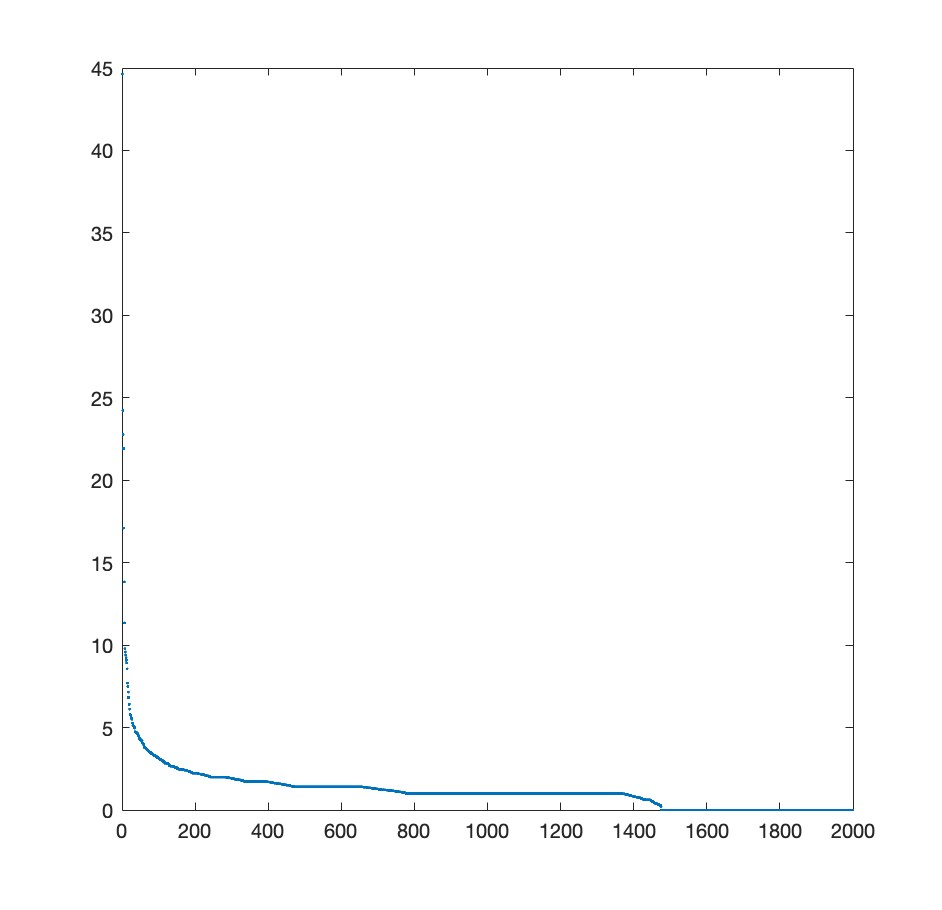
\includegraphics[width=0.8\textwidth]{s.jpg}
                \caption{Singular values of the first 2000 columns of $\mathbf{M}$}
            \end{figure}
        \end{column}
    \end{columns}
\end{frame}

% second page
% Introduce two papers :
% LORA: LOW-RANK ADAPTATION OF LARGE LANGUAGE MODELS
% INTRINSIC DIMENSIONALITY EXPLAINS THE EFFECTIVENESS OF LANGUAGE MODEL FINE-TUNING
\begin{frame}
    \frametitle{Low-rank adaptation of large language models \\ Intrinsic dimensionality explains the effectiveness of language model fine-tuning}

    \begin{itemize}
        \item The weight matrix may not be low-rank, but the fine-tuned difference matrix is low-rank.
        \item The first one proposed a method $ W' = W + \Delta W = W + BA$ to approximate the fine-tuned difference matrix.
        \item The second one proposed new interpretation of intrinsic dimensionality, which is the minimal description length of the fine-tuning task within the framework of the pre-trained model. Under this interpretation, the paper demonstrates how the process of pre-training implicitly optimizes the description length over the average of NLP tasks, even though the pre-trained model does not have direct access to those same tasks.
    \end{itemize}
\end{frame}

\end{document}